\apendice{Manual de especificación de diseño}

Este apartado describe la estructura interna y el flujo funcional de la aplicación web desarrollada en el proyecto. Aunque la aplicación no sigue una arquitectura orientada a objetos compleja, se ha estructurado en componentes claramente diferenciados que permiten comprender su funcionamiento y facilitar su mantenimiento. Para ello, se incluyen dos representaciones visuales que ilustran cómo se organizan los elementos del sistema y cómo se comporta la herramienta desde la entrada del usuario hasta la presentación de resultados.


\section{Diseño arquitectónico}

El siguiente esquema representa la arquitectura funcional de la aplicación web, organizada en capas lógicas. Esta representación se centra exclusivamente en los módulos que componen la aplicación desarrollada (basada en Streamlit), sin incluir otros aspectos metodológicos del TFG como el análisis previo de datos o la evaluación del modelo.


\begin{figure}[H]
    \centering
    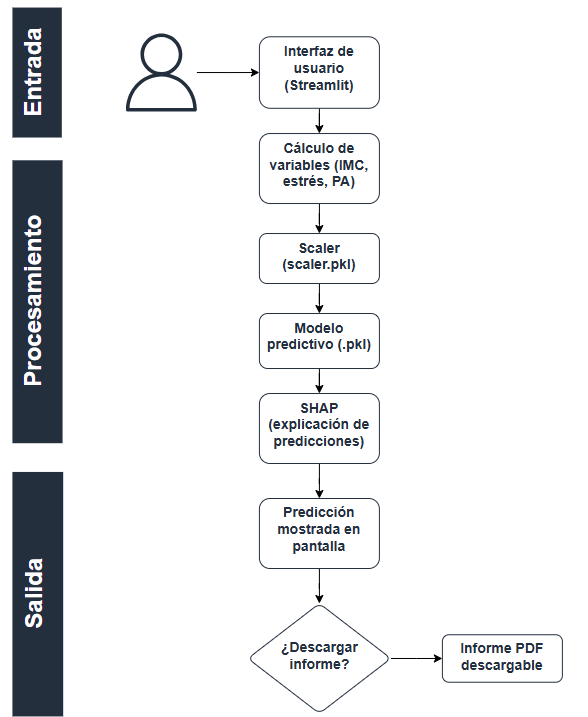
\includegraphics[width=0.75\linewidth]{img/diseño_arquit.png}
    \caption{Diseño arquitectónico funcional de la aplicación, estructurado en capas lógicas de entrada, procesamiento y salida.}
    \label{fig:diseño-arquitectonico}
\end{figure}


\section{Diagrama de flujo del funcionamiento}

El diagrama siguiente representa el flujo interno de la aplicación, desde el momento en que el usuario accede al sistema hasta que se genera la predicción y, opcionalmente, el informe en PDF. Este flujo refleja la secuencia real de operaciones ejecutadas en la aplicación al recibir datos de entrada, realizar la predicción mediante el modelo entrenado y generar las salidas asociadas, como la explicación con SHAP y el informe en PDF.


\begin{figure}[H]
    \centering
    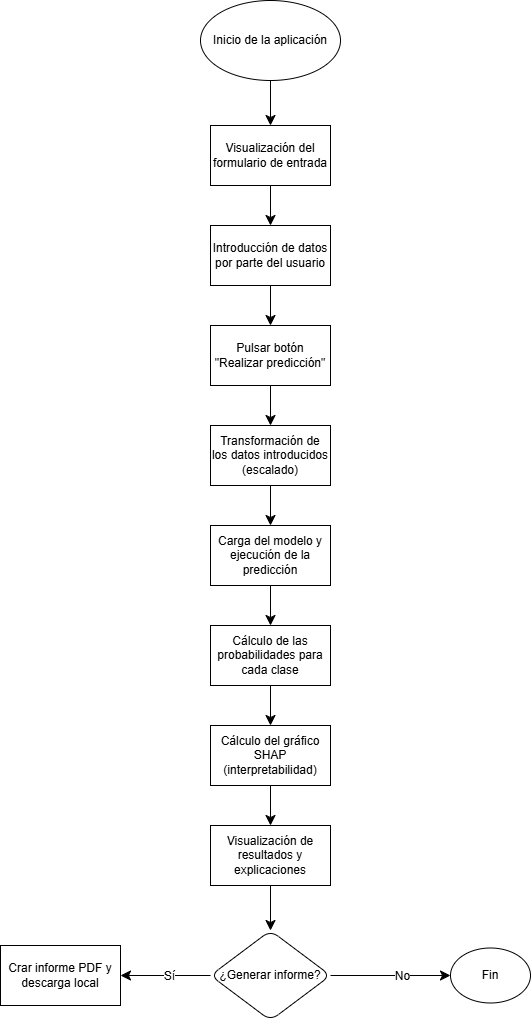
\includegraphics[width=0.85\linewidth]{img/diagramaApp.png}
    \caption{Diagrama de flujo del funcionamiento interno de la aplicación web.}
    \label{fig:diagrama}
\end{figure}

Ambas representaciones permiten visualizar de forma clara la lógica interna del sistema y servirán de referencia para su futura adaptación, mejora o extensión por parte de otros desarrolladores o equipos clínicos.
